\documentclass[final,12pt,]{CSUNthesis}

\author{Author Name}

\usepackage{graphicx}
\usepackage{cite}
\newcommand\citep{\cite}
\usepackage{listings}

\title{Thesis Title}
\references{plain}{bibliography}
\committee
{Chair Member}
{2nd Member}
{3rd Member}

\submitted{February}{2017}

\abstract{Abstract goes here}

\degree{Master of Science}{Psychology}

\defense{Monday}{February 13th}{3:30PM}{LO134}

\copyrightyear{2017}

\dedication{Dedication goes here}

\preface{Preface goes here}

\acknowledgement{Acknowledgement goes here}

\contact{\href{mailto:author@csun.edu}{\nolinkurl{author@csun.edu}}}

\collaboration{Author Two}

\begin{document}

\chapter{The First Chapter}\label{the-first-chapter}

\section{The First Section}\label{the-first-section}

We are writing this using LaTeX \citep{latex}.

R Markdown is a much simpler language that compiles to LaTeX. We can do
all sorts of things without the hassle of LaTeX:

\emph{italics} and \textbf{bold}.

\begin{itemize}
\item
  A thing
\item
  Another thing
\item
  Another another thing
\end{itemize}

\begin{enumerate}
\def\labelenumi{\arabic{enumi}.}
\item
  First Thing
\item
  Second thing
\end{enumerate}

\begin{quote}
``Quotes look better in blocks.'' -Someone
\end{quote}

\chapter{The Second Chapter}\label{the-second-chapter}

\section{The First Section in the Second
Chapter}\label{the-first-section-in-the-second-chapter}

We can include raw LaTeX:

\[ \sum_{i=1}^{\infty} \frac{1}{i} \leq \infty \]

We can also include inline LaTeX like so: \(e^{i \pi}=-1\)

We can also add code from various programming languages.

\subsubsection{R}\label{r}

\begin{lstlisting}[language=
R
]
x <- rnorm(10, 0, 1)
2+2
\end{lstlisting}

\begin{verbatim}
## [1] 4
\end{verbatim}

\begin{lstlisting}[language=
R
]
plot(x)
\end{lstlisting}

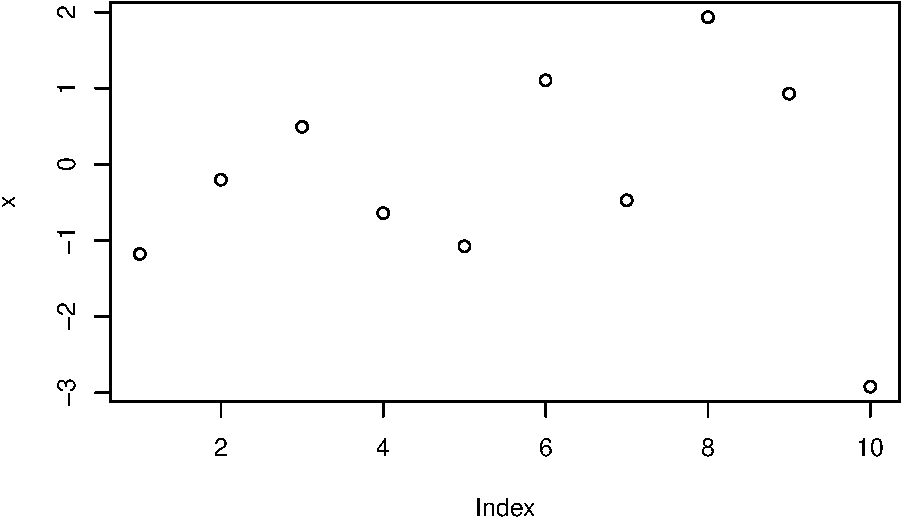
\includegraphics{skeleton_files/figure-latex/unnamed-chunk-1-1.pdf}

\subsubsection{Haskell}\label{haskell}

\begin{lstlisting}[language=
haskell
]
[x | x <- [1..10], odd x]
\end{lstlisting}

\begin{verbatim}
## [1,3,5,7,9]
\end{verbatim}

\subsubsection{Python}\label{python}

\begin{lstlisting}[language=
python
]
x = 'hello, python world!'
print(x.split(' '))
\end{lstlisting}

\begin{verbatim}
## ['hello,', 'python', 'world!']
\end{verbatim}

\end{document}
